\documentclass[12pt,a4paper]{article}

\usepackage[utf8]{inputenc}
\usepackage[T1]{fontenc}
\usepackage{lmodern}
\usepackage{amsmath,amssymb}
\usepackage{geometry}
\usepackage{hyperref}
\usepackage{xcolor}
\usepackage{listings}
\usepackage{microtype}
\usepackage{tikz}
\usepackage{float} % Provides [H] to keep each diagram directly below its heading
\usetikzlibrary{arrows.meta,positioning,shapes.geometric,fit,calc,shapes.symbols,decorations.pathreplacing}

\geometry{margin=1in}
\hypersetup{colorlinks=true,linkcolor=blue,urlcolor=blue,citecolor=blue}

\definecolor{codegray}{RGB}{245,245,245}
\definecolor{codeblue}{RGB}{25,70,130}
\lstset{
  language=C++,
  basicstyle=\ttfamily\small,
  keywordstyle=\color{codeblue}\bfseries,
  commentstyle=\color{gray}\itshape,
  stringstyle=\color{red!55!black},
  numbers=left,
  numberstyle=\tiny\color{gray},
  stepnumber=1,
  numbersep=8pt,
  backgroundcolor=\color{codegray},
  frame=single,
  breaklines=true,
  showstringspaces=false,
  tabsize=4,
  columns=fullflexible
}



\tikzset{
  block/.style={draw,rounded corners,align=center,minimum width=3.0cm,minimum height=0.8cm,fill=blue!5},
  smallblock/.style={draw,rounded corners,align=center,minimum width=2.2cm,minimum height=0.7cm,fill=blue!5},
  decision/.style={draw,diamond,aspect=2,align=center,inner sep=2pt,fill=orange!10},
  umlclass/.style={draw,rectangle,align=left,text width=4.0cm,font=\small},
  arrow/.style={-{Stealth[length=2.2mm]},thick}
}

\title{Regex Evaluator Using NFA and DFA\\[0.5em]{\large CS3104 Mini Project Final Report}}
\author{Konduru Navadeep, Alavala Prathap Reddy\\Roll Number: \textit{[251132,251107]}}
\date{}
\begin{document}
\maketitle
\tableofcontents
\clearpage



\section{Introduction and Problem Statement}
Regular expressions provide a compact way to describe patterns in strings. Checking whether a string follows a regular expression is a common task in text processing, input validation, lexical analysis, and compiler design. A full-featured production regex library can be complex and may hide the algorithms used to perform matching.

This project implements a lightweight regular-expression evaluator in C++. The user supplies a regular expression and a test string. The program parses the expression into a syntax tree, builds a Non-deterministic Finite Automaton (NFA), converts the NFA into a Deterministic Finite Automaton (DFA), and uses the DFA to decide whether the entire input string is accepted. The result is printed as \texttt{ACCEPT} or \texttt{REJECT}.

The main problem addressed is to demonstrate the internal stages of regex evaluation using object-oriented programming (OOP), finite-automata algorithms, and the C++ Standard Template Library (STL), rather than relying on a built-in regex library.

\section{Scope and Feature Set}
The implementation focuses on a small and understandable subset of regular-expression syntax.
\begin{itemize}
    \item \textbf{Literal characters:} matches a character such as \texttt{a}.
    \item \textbf{Concatenation:} matches expressions in sequence, for example \texttt{abc}.
    \item \textbf{Union:} the \texttt{|} operator represents alternatives, for example \texttt{a|b}.
    \item \textbf{Kleene star:} the \texttt{*} operator represents zero or more repetitions, for example \texttt{a*}.
    \item \textbf{Grouping:} parentheses group expressions, for example \texttt{(a|b)*}.
    \item \textbf{Automata construction:} builds an NFA using Thompson's construction and converts it to a DFA using subset construction.
    \item \textbf{Input validation:} rejects malformed expressions handled by the parser, including unmatched parentheses, a trailing union operator, a standalone star, repeated stars, and empty groups.
    \item \textbf{Automated tests:} a PowerShell script compiles the C++ source files and checks 21 input cases against expected results.
\end{itemize}

The current implementation is limited. Operators such as \texttt{+}, \texttt{?}, character classes, escape sequences, and wildcard matching are outside its current scope.

\section{Object-Oriented Architecture}
The program separates parsing, syntax-tree representation, NFA construction, NFA operations, DFA construction, and simulation into individual classes. This separation makes the implementation easier to understand, test, and extend.

\subsection{Class Design and Associations}
\texttt{RegexNode} is the abstract base class for syntax-tree nodes. \texttt{LiteralNode}, \texttt{ConcatNode}, \texttt{UnionNode}, and \texttt{StarNode} derive from it. The parser produces a tree of these nodes. The NFA builder traverses the tree and creates NFA fragments. NFA and DFA state classes store transitions, while simulator classes perform matching.

\begin{figure}[H]
\centering
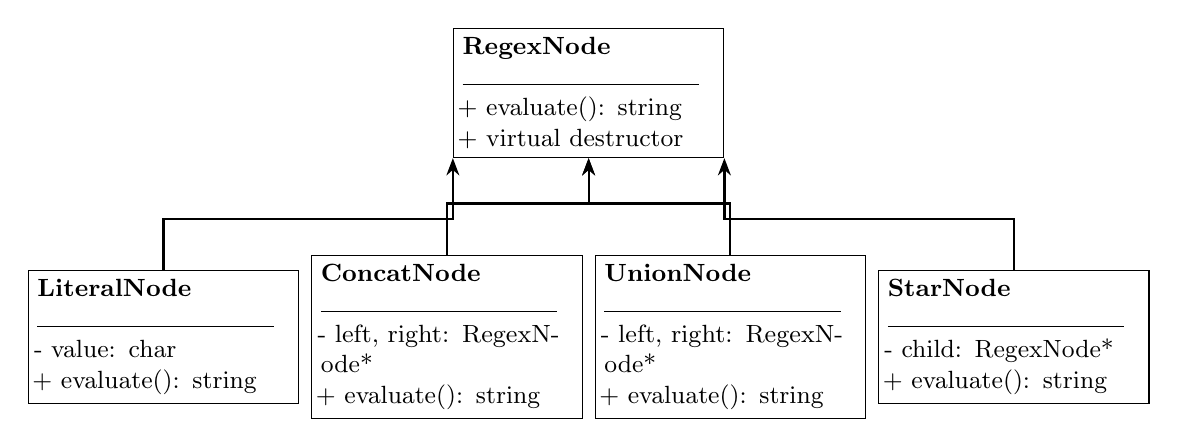
\begin{tikzpicture}
  \node[umlclass,text width=3.2cm] (base) at (0,0) {\textbf{RegexNode}\\\rule{3.0cm}{0.3pt}\\+ evaluate(): string\\+ virtual destructor};
  \node[umlclass,text width=3.2cm] (lit) at (-5.4,-3.1) {\textbf{LiteralNode}\\\rule{3.0cm}{0.3pt}\\- value: char\\+ evaluate(): string};
  \node[umlclass,text width=3.2cm] (con) at (-1.8,-3.1) {\textbf{ConcatNode}\\\rule{3.0cm}{0.3pt}\\- left, right: RegexNode*\\+ evaluate(): string};
  \node[umlclass,text width=3.2cm] (uni) at (1.8,-3.1) {\textbf{UnionNode}\\\rule{3.0cm}{0.3pt}\\- left, right: RegexNode*\\+ evaluate(): string};
  \node[umlclass,text width=3.2cm] (star) at (5.4,-3.1) {\textbf{StarNode}\\\rule{3.0cm}{0.3pt}\\- child: RegexNode*\\+ evaluate(): string};
  \draw[arrow] (lit.north) -- ++(0,0.65) -| (base.south west);
  \draw[arrow] (con.north) -- ++(0,0.65) -| (base.south);
  \draw[arrow] (uni.north) -- ++(0,0.65) -| (base.south);
  \draw[arrow] (star.north) -- ++(0,0.65) -| (base.south east);
\end{tikzpicture}
\caption{Simplified class diagram for the syntax-tree node hierarchy.}
\label{fig:class-diagram}
\end{figure}

\subsection{OOP Principles}
\begin{itemize}
    \item \textbf{Abstraction:} \texttt{RegexNode} defines a common interface through the pure virtual function \texttt{evaluate()}.
    \item \textbf{Inheritance:} the literal, concatenation, union, and star nodes inherit from \texttt{RegexNode}.
    \item \textbf{Polymorphism:} derived node implementations provide their own \texttt{evaluate()} behaviour and can be handled through a base-class pointer.
    \item \textbf{Encapsulation:} node data and automaton state/transition information are maintained within their respective classes and exposed through class interfaces.
    \item \textbf{Modularity:} parser, builders, operations, and simulators have separate responsibilities.
\end{itemize}

\subsection{Abstract Base Class and Virtual Function}
The following excerpt shows the common interface used by syntax-tree nodes.
\begin{lstlisting}
class RegexNode {
public:
    virtual ~RegexNode() = default;
    virtual std::string evaluate() = 0;
};
\end{lstlisting}
The assignment of \texttt{= 0} makes \texttt{evaluate()} a pure virtual function, so \texttt{RegexNode} is abstract and cannot be instantiated directly. The virtual destructor allows derived objects to be safely destroyed through a base-class pointer.

\section{System Architecture and Design}
The processing pipeline consists of the following stages:
\begin{enumerate}
    \item Read the regular expression and input string from the console.
    \item Parse the expression using recursive-descent parsing and construct a syntax tree.
    \item Convert the syntax tree into an NFA using Thompson's construction.
    \item Use epsilon-closure and move operations to determine reachable NFA states.
    \item Convert the NFA into a DFA through subset construction.
    \item Simulate the DFA on the input string and print the final result.
\end{enumerate}

\begin{figure}[H]
\centering
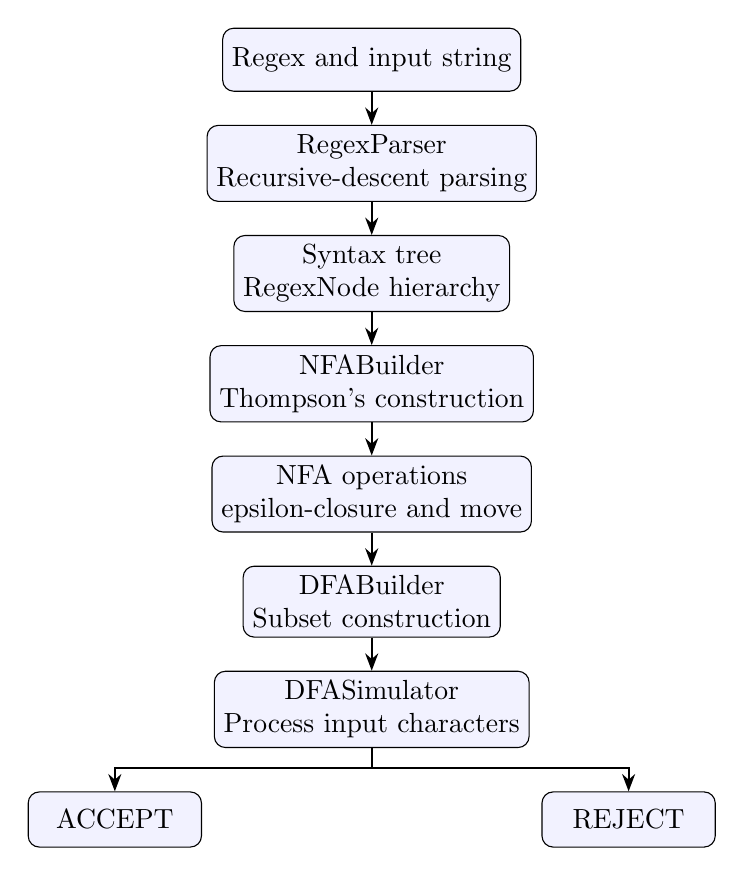
\begin{tikzpicture}[node distance=0.42cm]
  \node[block] (input) {Regex and input string};
  \node[block,below=of input] (parser) {RegexParser\\Recursive-descent parsing};
  \node[block,below=of parser] (tree) {Syntax tree\\RegexNode hierarchy};
  \node[block,below=of tree] (nfa) {NFABuilder\\Thompson's construction};
  \node[block,below=of nfa] (ops) {NFA operations\\epsilon-closure and move};
  \node[block,below=of ops] (dfa) {DFABuilder\\Subset construction};
  \node[block,below=of dfa] (sim) {DFASimulator\\Process input characters};
  \node[smallblock,below left=0.55cm and 0.15cm of sim] (accept) {ACCEPT};
  \node[smallblock,below right=0.55cm and 0.15cm of sim] (reject) {REJECT};
  \foreach \a/\b in {input/parser,parser/tree,tree/nfa,nfa/ops,ops/dfa,dfa/sim} \draw[arrow] (\a) -- (\b);
  \draw[arrow] (sim.south) -- ++(0,-0.25) -| (accept.north);
  \draw[arrow] (sim.south) -- ++(0,-0.25) -| (reject.north);
\end{tikzpicture}
\caption{High-level architecture of the Regex Evaluator.}
\label{fig:architecture}
\end{figure}

\subsection{Use Case Diagram}
The primary actor is the user, who supplies a regular expression and a string to test. The system validates/parses the expression, evaluates the string, and displays the result.
\begin{figure}[H]
\centering
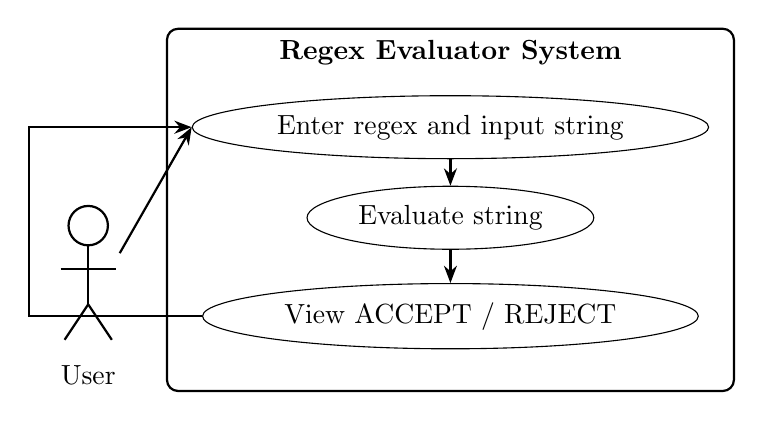
\begin{tikzpicture}[node distance=0.8cm]
  \draw[rounded corners,thick] (1.0,-0.1) rectangle (8.2,4.5);
  \node[font=\bfseries] at (4.6,4.2) {Regex Evaluator System};
  \draw[thick] (0,2.0) circle (0.25);
  \draw[thick] (0,1.75) -- (0,1.0);
  \draw[thick] (-0.35,1.45) -- (0.35,1.45);
  \draw[thick] (0,1.0) -- (-0.3,0.55);
  \draw[thick] (0,1.0) -- (0.3,0.55);
  \node[below] at (0,0.35) {User};
  \node[draw,ellipse,minimum width=3.3cm,minimum height=0.8cm] (enter) at (4.6,3.25) {Enter regex and input string};
  \node[draw,ellipse,minimum width=3.3cm,minimum height=0.8cm] (evaluate) at (4.6,2.1) {Evaluate string};
  \node[draw,ellipse,minimum width=3.3cm,minimum height=0.8cm] (result) at (4.6,0.85) {View ACCEPT / REJECT};
  \draw[arrow] (0.4,1.65) -- (enter.west);
  \draw[arrow] (enter) -- (evaluate);
  \draw[arrow] (evaluate) -- (result);
  \draw[arrow] (result.west) -- ++(-2.2,0) -- ++(0,2.4) -- (enter.west);
\end{tikzpicture}
\caption{Use case diagram.}
\label{fig:usecase}
\end{figure}

\subsection{Activity Diagram}
\begin{figure}[H]
\centering
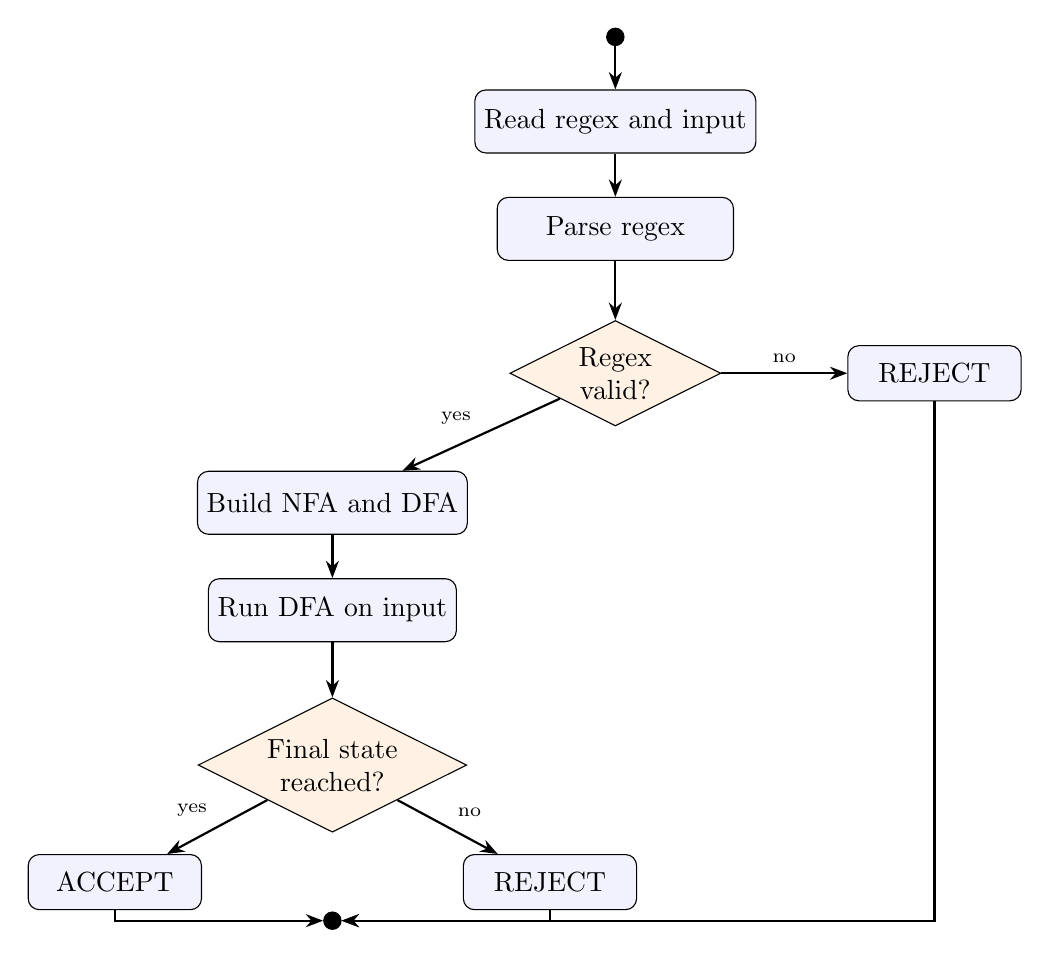
\begin{tikzpicture}[node distance=0.55cm]
  \node[draw,circle,fill=black,minimum size=0.22cm,inner sep=0pt] (start) {};
  \node[block,below=of start] (read) {Read regex and input};
  \node[block,below=of read] (parse) {Parse regex};
  \node[decision,below=0.75cm of parse] (valid) {Regex\\valid?};
  \node[block,below left=0.9cm and 1.2cm of valid] (build) {Build NFA and DFA};
  \node[block,below=of build] (match) {Run DFA on input};
  \node[decision,below=0.7cm of match] (final) {Final state\\reached?};
  \node[smallblock,below left=0.7cm and 0.8cm of final] (yes) {ACCEPT};
  \node[smallblock,below right=0.7cm and 0.8cm of final] (no) {REJECT};
  \node[smallblock,right=1.6cm of valid] (invalid) {REJECT};
  \node[draw,circle,fill=black,minimum size=0.22cm,inner sep=0pt,below=1.0cm of final] (end) {};
  \draw[arrow] (start) -- (read);
  \draw[arrow] (read) -- (parse);
  \draw[arrow] (parse) -- (valid);
  \draw[arrow] (valid) -- node[above left,font=\scriptsize] {yes} (build);
  \draw[arrow] (valid) -- node[above,font=\scriptsize] {no} (invalid);
  \draw[arrow] (build) -- (match);
  \draw[arrow] (match) -- (final);
  \draw[arrow] (final) -- node[above left,font=\scriptsize] {yes} (yes);
  \draw[arrow] (final) -- node[above right,font=\scriptsize] {no} (no);
  \draw[arrow] (yes) |- (end);
  \draw[arrow] (no) |- (end);
  \draw[arrow] (invalid) |- (end);
\end{tikzpicture}
\caption{Activity diagram for evaluating a regular expression.}
\label{fig:activity}
\end{figure}

\subsection{Sequence Diagram}
\begin{figure}[H]
\centering
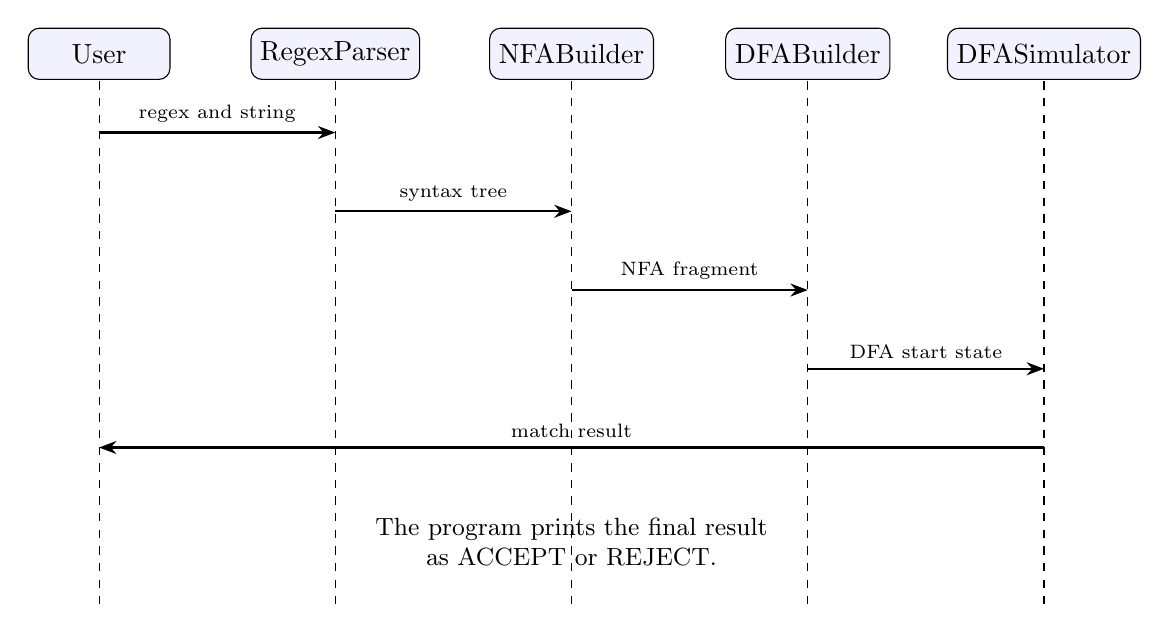
\begin{tikzpicture}[x=1cm,y=1cm]
  \node[draw,rounded corners,fill=blue!5,minimum width=1.8cm,minimum height=0.65cm] (user) at (0,0) {User};
  \node[draw,rounded corners,fill=blue!5,minimum width=2.0cm,minimum height=0.65cm] (parser) at (3,0) {RegexParser};
  \node[draw,rounded corners,fill=blue!5,minimum width=2.0cm,minimum height=0.65cm] (nfa) at (6,0) {NFABuilder};
  \node[draw,rounded corners,fill=blue!5,minimum width=2.0cm,minimum height=0.65cm] (dfa) at (9,0) {DFABuilder};
  \node[draw,rounded corners,fill=blue!5,minimum width=2.0cm,minimum height=0.65cm] (sim) at (12,0) {DFASimulator};
  \foreach \x in {0,3,6,9,12} \draw[dashed] (\x,-0.35) -- (\x,-7.0);
  \draw[arrow] (0,-1.0) -- node[above,sloped,font=\scriptsize] {regex and string} (3,-1.0);
  \draw[arrow] (3,-2.0) -- node[above,sloped,font=\scriptsize] {syntax tree} (6,-2.0);
  \draw[arrow] (6,-3.0) -- node[above,sloped,font=\scriptsize] {NFA fragment} (9,-3.0);
  \draw[arrow] (9,-4.0) -- node[above,sloped,font=\scriptsize] {DFA start state} (12,-4.0);
  \draw[arrow] (12,-5.0) -- node[above,sloped,font=\scriptsize] {match result} (0,-5.0);
  \node[align=center,font=\small] at (6,-6.2) {The program prints the final result\\as ACCEPT or REJECT.};
\end{tikzpicture}
\caption{Simplified sequence of interactions between the user and core components.}
\label{fig:sequence}
\end{figure}

\section{Core Algorithms}
\subsection{Recursive-Descent Parsing}
The parser processes the expression using a set of mutually cooperating functions. \texttt{parseExpression()} handles union, \texttt{parseTerm()} handles concatenation, \texttt{parseFactor()} handles the Kleene-star postfix operator, and \texttt{parsePrimary()} handles literals and parenthesized expressions. This structure captures the precedence of the supported operators: grouping and star bind more tightly than concatenation, which binds more tightly than union.

\subsection{Thompson's NFA Construction}
Thompson's construction creates an NFA fragment with a start state and an accepting state for each syntax-tree node.
\begin{itemize}
    \item For a literal, create two states and connect them using the literal character.
    \item For concatenation, connect the first fragment's accepting state to the second fragment's start using an epsilon transition.
    \item For union, create a new start and end state and use epsilon transitions to branch to either alternative and rejoin.
    \item For Kleene star, add epsilon transitions that allow the child fragment to be skipped or repeated.
\end{itemize}
In the implementation, the null character \texttt{'\\0'} represents an epsilon transition.

\subsection{NFA Operations and Subset Construction}
The epsilon-closure operation finds all states reachable using only epsilon transitions. The move operation finds states reachable on a given input symbol. During subset construction, each DFA state represents a set of NFA states. For each symbol in the NFA alphabet, the builder computes move followed by epsilon-closure. A DFA state is accepting when its represented set contains at least one accepting NFA state.

\subsection{DFA Simulation}
The DFA simulator starts from the DFA start state and processes the input from left to right. For each character, it follows the corresponding transition. If a required transition is absent, the string is rejected. After the entire string is consumed, the string is accepted only if the current DFA state is final. This performs full-string matching rather than searching for a substring.

\section{Selected Code Snippets}
\subsection{DFA Matching}
The following excerpt illustrates the deterministic matching stage.
\begin{lstlisting}
bool DFASimulator::matches(DFAState* start,
                           const std::string& input) {
    DFAState* current = start;

    for (char symbol : input) {
        if (current->transitions.count(symbol) == 0)
            return false;
        current = current->transitions[symbol];
    }

    return current->isFinal;
}
\end{lstlisting}
The transition lookup is deterministic: for each input symbol there is at most one next state. A missing transition immediately rejects the string, while the final-state check determines the result after all characters have been processed.

\subsection{NFA-to-DFA State Reuse}
Subset construction avoids creating duplicate DFA states by checking whether a state already represents the same set of NFA states.
\begin{lstlisting}
DFAState* DFABuilder::findState(
    const std::vector<DFAState*>& states,
    const std::set<NFAState*>& nfaStates) {
    for (DFAState* state : states) {
        if (state->nfaStates == nfaStates)
            return state;
    }
    return nullptr;
}
\end{lstlisting}
This check is important because the same set of NFA states may be reached by different input paths. Reusing the existing DFA state prevents duplicate states from being created.

\section{Formal Specification of the Supported Language}
This section defines the exact subset of regular expressions implemented by the evaluator. A regular expression is interpreted as a pattern for the entire input string. It is not a substring-search engine: every input character must be consumed and the final automaton state must be accepting.

\subsection{Supported operators and examples}
\begin{table}[htbp]
\centering
\caption{Supported regular-expression syntax.}
\label{tab:operators}
\small
\begin{tabular}{|p{2.8cm}|p{4.4cm}|p{6.0cm}|}
\hline
\textbf{Syntax} & \textbf{Meaning} & \textbf{Example and interpretation} \\
\hline
Literal & A character matches itself. & \texttt{a} accepts only the one-character string \texttt{a}. \\
\hline
Concatenation & Expressions occur in sequence. & \texttt{abc} accepts the three-character string \texttt{abc}. \\
\hline
Union \texttt{|} & Either the left or right expression may match. & \texttt{a|b} accepts \texttt{a} or \texttt{b}. \\
\hline
Kleene star \texttt{*} & The preceding factor occurs zero or more times. & \texttt{a*} accepts the empty string, \texttt{a}, \texttt{aa}, and so on. \\
\hline
Parentheses & Group an expression and control precedence. & \texttt{(a|b)*} accepts any string made from \texttt{a} and \texttt{b}, including empty input. \\
\hline
\end{tabular}
\end{table}

\subsection{Operator precedence and parser grammar}
The parser's structure gives grouping and the postfix star the highest precedence, concatenation the next highest precedence, and union the lowest precedence. Concatenation is implicit: there is no concatenation symbol in the input.

A simplified grammar for the implemented syntax is:
\begin{align*}
\text{Expression} &\rightarrow \text{Term}\,(\texttt{|}\,\text{Term})^* \\
\text{Term} &\rightarrow \text{Factor}^+ \\
\text{Factor} &\rightarrow \text{Primary}\,(\texttt{*})? \\
\text{Primary} &\rightarrow \text{Literal}\mid\texttt{(}\,\text{Expression}\,\texttt{)}
\end{align*}
This grammar is a conceptual description of valid non-empty expressions. The implementation also has explicit checks for malformed forms such as a trailing union, a standalone star, an empty group, repeated stars, and unbalanced parentheses. Empty regular expressions are handled separately in \texttt{main.cpp}: the current program accepts an empty input when the regex is empty and rejects non-empty input for an empty regex.

\subsection{Recursive-descent parser responsibilities}
\begin{table}[htbp]
\centering
\caption{Parser functions and their responsibilities.}
\begin{tabular}{|l|p{9.5cm}|}
\hline
\textbf{Function} & \textbf{Responsibility} \\
\hline
\texttt{parse()} & Starts parsing, checks for a valid root node, and verifies that the entire expression was consumed. \\
\hline
\texttt{parseExpression()} & Parses a term and combines subsequent terms separated by \texttt{|} into \texttt{UnionNode} objects. \\
\hline
\texttt{parseTerm()} & Parses adjacent factors and combines them into \texttt{ConcatNode} objects. \\
\hline
\texttt{parseFactor()} & Parses a primary expression and optionally wraps it in a \texttt{StarNode}. \\
\hline
\texttt{parsePrimary()} & Parses a literal or a parenthesized expression; rejects invalid leading operators and empty groups. \\
\hline
\end{tabular}
\end{table}

\section{Detailed Object Model}
\subsection{Responsibilities of the main classes}
The program is organized around a pipeline of classes, each with one main responsibility. This separation makes it easier to test and explain the implementation.
\begin{table}[htbp]
\centering
\caption{Class responsibility reference.}
\small
\begin{tabular}{|p{3.0cm}|p{9.7cm}|}
\hline
\textbf{Class} & \textbf{Responsibility} \\
\hline
\texttt{RegexNode} & Abstract syntax-tree interface; declares the pure virtual \texttt{evaluate()} function and virtual destructor. \\
\hline
\texttt{LiteralNode} & Stores one literal character and returns its one-character string representation. \\
\hline
\texttt{ConcatNode} & Holds left and right child nodes and evaluates them in sequence. \\
\hline
\texttt{UnionNode} & Holds two alternatives and represents their union using \texttt{|}. \\
\hline
\texttt{StarNode} & Holds a child node and represents zero or more repetitions of that child. \\
\hline
\texttt{RegexParser} & Uses recursive-descent functions to validate and convert the input expression into a syntax tree. \\
\hline
\texttt{NFAState} & Stores a state identifier, final-state flag, and a list of symbol/destination transitions. \\
\hline
\texttt{NFAFragment} & Groups an NFA start state and end state so recursive construction can return a complete fragment. \\
\hline
\texttt{NFABuilder} & Recursively traverses the syntax tree and constructs NFA fragments using Thompson's construction. \\
\hline
\texttt{NFAOperations} & Provides epsilon-closure and move operations over sets of NFA states. \\
\hline
\texttt{NFASimulator} & Simulates an NFA by updating the reachable set of states for each input symbol. \\
\hline
\texttt{DFAState} & Represents a DFA state, the NFA-state subset associated with it, its final flag, and deterministic transitions. \\
\hline
\texttt{DFABuilder} & Converts the NFA to a DFA using subset construction and reuses existing subset states. \\
\hline
\texttt{DFASimulator} & Reads the input one character at a time, follows DFA transitions, and returns a Boolean result. \\
\hline
\end{tabular}
\end{table}

\subsection{Expanded class relationship diagram}
The following diagram complements the syntax-tree inheritance diagram in Figure~\ref{fig:class-diagram}. It shows the collaboration between the parser, automata builders, state objects, and simulators. Solid inheritance arrows in the syntax-tree diagram indicate an \emph{is-a} relationship; the arrows below indicate use or construction relationships.
\begin{figure}[H]
\centering
\resizebox{\textwidth}{!}{%
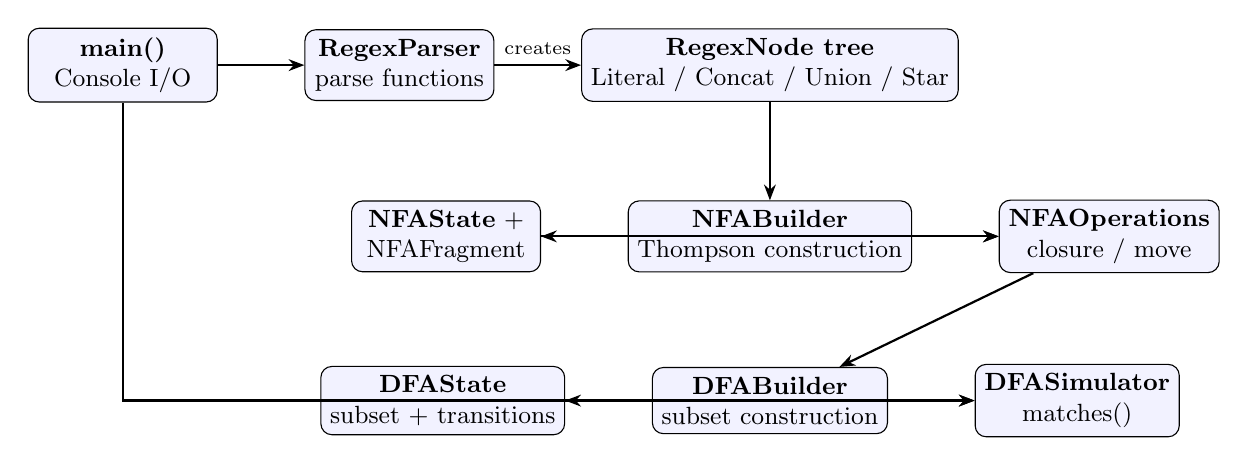
\begin{tikzpicture}[node distance=1.0cm and 1.1cm, every node/.style={font=\small},
  c/.style={draw,rounded corners,align=center,minimum width=2.4cm,minimum height=0.75cm,fill=blue!5},
  rel/.style={-{Stealth[length=2mm]},thick}]
  \node[c] (main) {\textbf{main()}\\Console I/O};
  \node[c,right=of main] (parser) {\textbf{RegexParser}\\parse functions};
  \node[c,right=of parser] (tree) {\textbf{RegexNode tree}\\Literal / Concat / Union / Star};
  \node[c,below=1.25cm of tree] (nfa) {\textbf{NFABuilder}\\Thompson construction};
  \node[c,left=of nfa] (nfastate) {\textbf{NFAState} +\\NFAFragment};
  \node[c,right=of nfa] (ops) {\textbf{NFAOperations}\\closure / move};
  \node[c,below=1.2cm of nfa] (dfab) {\textbf{DFABuilder}\\subset construction};
  \node[c,left=of dfab] (dfastate) {\textbf{DFAState}\\subset + transitions};
  \node[c,right=of dfab] (sim) {\textbf{DFASimulator}\\matches()};
  \draw[rel] (main) -- (parser);
  \draw[rel] (parser) -- node[above,font=\scriptsize]{creates} (tree);
  \draw[rel] (tree) -- (nfa);
  \draw[rel] (nfa) -- (nfastate);
  \draw[rel] (nfa) -- (ops);
  \draw[rel] (nfastate) -- (ops);
  \draw[rel] (ops) -- (dfab);
  \draw[rel] (dfab) -- (dfastate);
  \draw[rel] (dfab) -- (sim);
  \draw[rel] (main.south) |- (sim.west);
\end{tikzpicture}%
}
\caption{Collaboration diagram for the main implementation components.}
\label{fig:component-class-map}
\end{figure}

\subsection{Object-oriented design discussion}
\textbf{Abstraction.} The abstract \texttt{RegexNode} class exposes the common \texttt{evaluate()} operation without specifying one representation for every expression. 

\textbf{Inheritance.} \texttt{LiteralNode}, \texttt{ConcatNode}, \texttt{UnionNode}, and \texttt{StarNode} inherit from \texttt{RegexNode}. They can therefore be handled through the common base type.

\textbf{Polymorphism.} Each derived node overrides \texttt{evaluate()}. The NFA builder identifies the concrete node type using \texttt{dynamic\_cast} and delegates construction to the matching builder function. This implementation uses runtime type checks in the builder; the virtual function is still part of the syntax-tree interface.

\textbf{Encapsulation.} The syntax-tree child pointers and literal values are private. Public getter functions expose the child nodes needed by the builder. State transitions are stored in state objects. Some state fields are public in the current implementation, so encapsulation is applied selectively rather than uniformly.

\textbf{Composition and association.} A concatenation node refers to two child nodes, a union node refers to two alternatives, and a star node refers to one child. An NFA fragment groups a start and end state. These are logical ownership/association relationships in the current pointer-based design; the code does not use smart pointers to enforce ownership automatically.

\section{Finite Automata: Visual Construction Walkthrough}
This section uses small diagrams to explain the algorithmic ideas. The drawings are explanatory TikZ figures created in LaTeX, not screenshots of diagrams from an external editor.

\subsection{NFA fragment for a literal}
For a literal \texttt{a}, Thompson's construction creates a start state, one character transition, and a final state.
\begin{figure}[H]
\centering
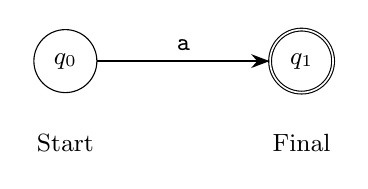
\begin{tikzpicture}[>=Stealth, every node/.style={font=\small}]
  \node[circle,draw,minimum size=8mm] (q0) at (0,0) {$q_0$};
  \node[circle,draw,double,minimum size=8mm] (q1) at (3,0) {$q_1$};
  \draw[->,thick] (q0) -- node[above]{\texttt{a}} (q1);
  \node[below=0.4cm of q0] {Start};
  \node[below=0.4cm of q1] {Final};
\end{tikzpicture}
\caption{NFA fragment for the literal expression \texttt{a}.}
\label{fig:nfa-literal}
\end{figure}

\subsection{NFA fragment for union}
For \texttt{a|b}, a new start state has epsilon transitions to both literal fragments. Their accepting paths join at a new final state. The symbol \texttt{\textbackslash epsilon} means the automaton can move without consuming an input character; in the C++ code this is represented by the null character \texttt{'\\0'}.
\begin{figure}[H]
\centering
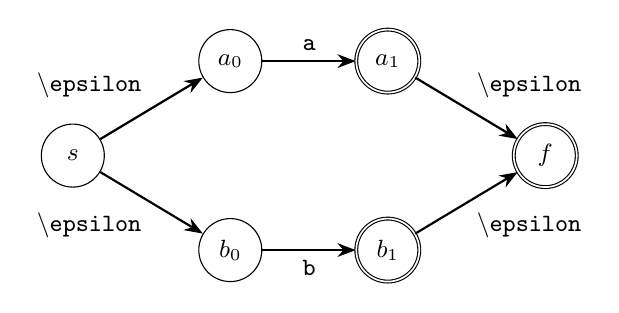
\begin{tikzpicture}[>=Stealth, every node/.style={font=\small}]
  \node[circle,draw,minimum size=8mm] (s) at (0,0) {$s$};
  \node[circle,draw,minimum size=8mm] (a0) at (2,1.2) {$a_0$};
  \node[circle,draw,double,minimum size=8mm] (a1) at (4,1.2) {$a_1$};
  \node[circle,draw,minimum size=8mm] (b0) at (2,-1.2) {$b_0$};
  \node[circle,draw,double,minimum size=8mm] (b1) at (4,-1.2) {$b_1$};
  \node[circle,draw,double,minimum size=8mm] (f) at (6,0) {$f$};
  \draw[->,thick] (s) -- node[above left]{\texttt{\textbackslash epsilon}} (a0);
  \draw[->,thick] (s) -- node[below left]{\texttt{\textbackslash epsilon}} (b0);
  \draw[->,thick] (a0) -- node[above]{\texttt{a}} (a1);
  \draw[->,thick] (b0) -- node[below]{\texttt{b}} (b1);
  \draw[->,thick] (a1) -- node[above right]{\texttt{\textbackslash epsilon}} (f);
  \draw[->,thick] (b1) -- node[below right]{\texttt{\textbackslash epsilon}} (f);
\end{tikzpicture}
\caption{Conceptual Thompson NFA structure for union \texttt{a|b}.}
\label{fig:nfa-union}
\end{figure}

\subsection{NFA fragment for Kleene star}
For \texttt{a*}, epsilon transitions permit zero repetitions by bypassing the child fragment, or one or more repetitions by returning from the child's accepting state to the child start. An additional epsilon path exits to the new final state.
\begin{figure}[H]
\centering
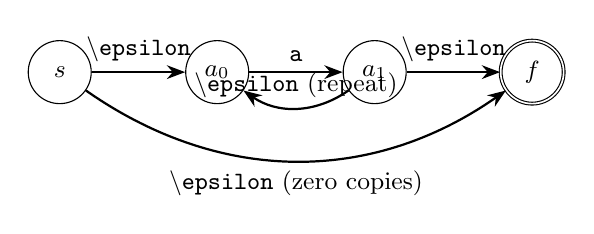
\begin{tikzpicture}[>=Stealth, every node/.style={font=\small}]
  \node[circle,draw,minimum size=8mm] (s) at (0,0) {$s$};
  \node[circle,draw,minimum size=8mm] (a0) at (2,0) {$a_0$};
  \node[circle,draw,minimum size=8mm] (a1) at (4,0) {$a_1$};
  \node[circle,draw,double,minimum size=8mm] (f) at (6,0) {$f$};
  \draw[->,thick] (s) -- node[above]{\texttt{\textbackslash epsilon}} (a0);
  \draw[->,thick] (a0) -- node[above]{\texttt{a}} (a1);
  \draw[->,thick] (a1) to[bend left=35] node[above]{\texttt{\textbackslash epsilon} (repeat)} (a0);
  \draw[->,thick] (a1) -- node[above]{\texttt{\textbackslash epsilon}} (f);
  \draw[->,thick] (s) to[bend right=35] node[below]{\texttt{\textbackslash epsilon} (zero copies)} (f);
\end{tikzpicture}
\caption{Conceptual Thompson NFA structure for \texttt{a*}.}
\label{fig:nfa-star}
\end{figure}

\subsection{How epsilon-closure and move work}
Suppose the current reachable NFA state set is $S$. The epsilon-closure operation adds every state reachable from any state in $S$ using zero or more epsilon transitions. The move operation follows only transitions labelled with a selected input symbol.
\begin{align*}
\operatorname{move}(S,c) &= \{q'\mid q\in S\text{ and }q\xrightarrow{c}q'\},\\
\epsilon\text{-closure}(S) &= \{q'\mid q\text{ can reach }q'\text{ using only epsilon transitions}\}.
\end{align*}
The NFA simulator first calculates the epsilon-closure of the start state. For each input character, it applies \texttt{move()} and then epsilon-closure again. The NFA accepts if the fragment's final state remains in the set after all input characters are consumed.

\subsection{Subset construction: NFA states become DFA states}
The subset construction creates a DFA state for each reachable set of NFA states. The set is the identity of that DFA state. When a newly calculated subset already exists, the builder reuses it instead of creating a duplicate. This is why the implementation keeps the represented NFA subset inside each \texttt{DFAState} object.
\begin{figure}[H]
\centering
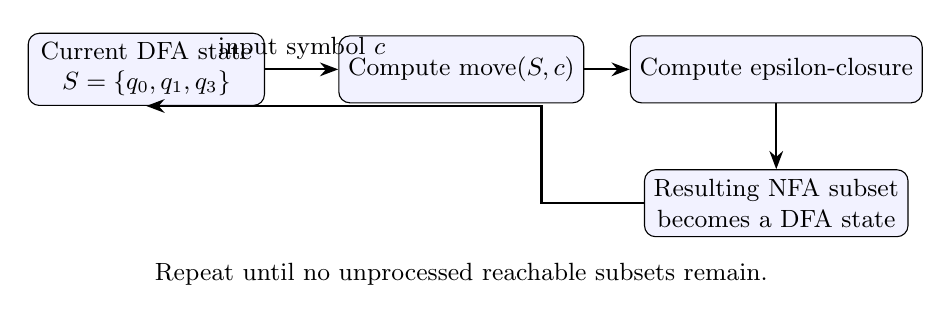
\begin{tikzpicture}[>=Stealth, every node/.style={font=\small}, box/.style={draw,rounded corners,align=center,minimum width=3.0cm,minimum height=0.85cm,fill=blue!5}]
  \node[box] (set) at (0,0) {Current DFA state\\$S=\{q_0,q_1,q_3\}$};
  \node[box] (move) at (4,0) {Compute $\operatorname{move}(S,c)$};
  \node[box] (closure) at (8,0) {Compute epsilon-closure};
  \node[box] (next) at (8,-1.7) {Resulting NFA subset\\becomes a DFA state};
  \draw[->,thick] (set) -- node[above]{input symbol $c$} (move);
  \draw[->,thick] (move) -- (closure);
  \draw[->,thick] (closure) -- (next);
  \draw[->,thick] (next.west) -- ++(-1.3,0) |- (set.south);
  \node[align=center] at (4,-2.6) {Repeat until no unprocessed reachable subsets remain.};
\end{tikzpicture}
\caption{The central step in subset construction. The state names are illustrative.}
\label{fig:subset-construction}
\end{figure}

\section{Worked Example: Evaluating \texttt{(a|b)*abb}}
The expression \texttt{(a|b)*abb} describes all strings over the alphabet \{\texttt{a},\texttt{b}\} that end with \texttt{abb}. The prefix \texttt{(a|b)*} can match any sequence of \texttt{a} and \texttt{b}, including an empty prefix; the suffix \texttt{abb} must occur at the end.

\subsection{Example input accepted}
Consider the input \texttt{abababb}. It can be divided into the prefix \texttt{abab} and suffix \texttt{abb}. The prefix is accepted by \texttt{(a|b)*}, and the remaining three characters match the required suffix. Therefore, the expected result is \texttt{ACCEPT}.

\begin{figure}[H]
\centering
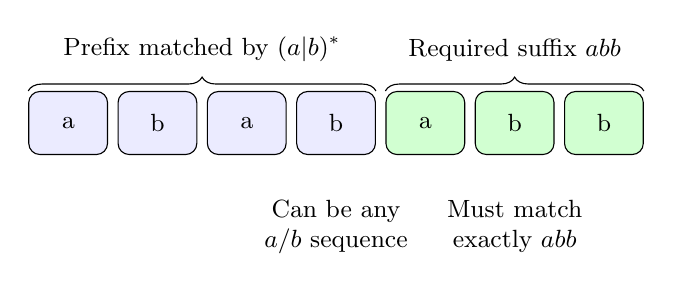
\begin{tikzpicture}[every node/.style={font=\small}]
  \node[draw,rounded corners,fill=blue!8,minimum width=1.0cm,minimum height=0.8cm] (c1) at (0,0) {a};
  \node[draw,rounded corners,fill=blue!8,minimum width=1.0cm,minimum height=0.8cm,right=0.12cm of c1] (c2) {b};
  \node[draw,rounded corners,fill=blue!8,minimum width=1.0cm,minimum height=0.8cm,right=0.12cm of c2] (c3) {a};
  \node[draw,rounded corners,fill=blue!8,minimum width=1.0cm,minimum height=0.8cm,right=0.12cm of c3] (c4) {b};
  \node[draw,rounded corners,fill=green!18,minimum width=1.0cm,minimum height=0.8cm,right=0.12cm of c4] (c5) {a};
  \node[draw,rounded corners,fill=green!18,minimum width=1.0cm,minimum height=0.8cm,right=0.12cm of c5] (c6) {b};
  \node[draw,rounded corners,fill=green!18,minimum width=1.0cm,minimum height=0.8cm,right=0.12cm of c6] (c7) {b};
  \draw[decorate,decoration={brace,amplitude=5pt}] (c1.north west) -- (c4.north east) node[midway,above=7pt] {Prefix matched by $(a|b)^*$};
  \draw[decorate,decoration={brace,amplitude=5pt}] (c5.north west) -- (c7.north east) node[midway,above=7pt] {Required suffix $abb$};
  \node[below=0.45cm of c4,align=center] {Can be any\\$a/b$ sequence};
  \node[below=0.45cm of c6,align=center] {Must match\\exactly $abb$};
\end{tikzpicture}
\caption{Visual decomposition of the accepted input \texttt{abababb}. Blue boxes represent the flexible prefix; green boxes represent the required suffix.}
\label{fig:worked-input}
\end{figure}

\subsection{Example input rejected}
The string \texttt{ab} is rejected because it ends before the required suffix \texttt{abb} has been completed. The string \texttt{abc} is also rejected: the character \texttt{c} is outside the alphabet described by this expression, and the required suffix is not matched. These examples demonstrate that a valid prefix alone is insufficient; the full input must reach a final DFA state.

\subsection{DFA simulation trace concept}
The DFA simulator stores a pointer to the current state. For every character, it looks up the matching transition. If the transition does not exist, the method returns \texttt{false}. If all characters are processed, the value of \texttt{isFinal} on the last state determines acceptance. The implementation does not display the internal state trace in the console; the following table is a conceptual trace of the simulator's decision process.
\begin{table}[htbp]
\centering
\caption{Conceptual decision trace for the accepted sample.}
\begin{tabular}{|p{2.1cm}|p{4.0cm}|p{5.2cm}|}
\hline
\textbf{Stage} & \textbf{Action} & \textbf{Reason} \\
\hline
Initial & Start at DFA start state. & No input has been consumed yet. \\
\hline
For each character & Follow the transition labelled by that character. & DFA state and input symbol determine at most one next state. \\
\hline
All characters consumed & Inspect the current state's final flag. & Acceptance depends on the complete input, not on a partial match. \\
\hline
Final check & Print \texttt{ACCEPT} if final; otherwise print \texttt{REJECT}. & This is the Boolean result returned by \texttt{DFASimulator::matches()}. \\
\hline
\end{tabular}
\end{table}

\section{Algorithm Pseudocode}
Pseudocode below summarizes the major algorithms without tying the explanation to C++ syntax.

\subsection{Recursive-descent parsing}
\begin{lstlisting}[language={},numbers=none]
parse():
    if expression is empty: return invalid/root-null
    root = parseExpression()
    if root is invalid: return invalid/root-null
    if not all characters were consumed: return invalid/root-null
    return root

parseExpression():
    node = parseTerm()
    while next character is '|':
        consume '|'
        right = parseTerm()
        if right is invalid: return invalid/root-null
        node = UnionNode(node, right)
    return node
\end{lstlisting}

\subsection{Thompson construction}
\begin{lstlisting}[language={},numbers=none]
build(node):
    if node is LiteralNode:
        create start and final states; connect by literal
    if node is ConcatNode:
        left = build(node.left); right = build(node.right)
        connect left.final to right.start by epsilon
        return (left.start, right.final)
    if node is UnionNode:
        build both alternatives
        create new start and final states
        epsilon-branch to both alternatives and rejoin
    if node is StarNode:
        build child fragment
        create new start and final states
        add epsilon paths for zero copies, repetition, and exit
\end{lstlisting}

\subsection{DFA matching}
\begin{lstlisting}[language={},numbers=none]
matches(start, input):
    current = start
    for each character c in input:
        if current has no transition on c:
            return false
        current = transition(current, c)
    return current.isFinal
\end{lstlisting}

\section{Complexity and Resource Considerations}
Let $m$ be the length of the regular expression and $n$ be the length of the input string. Parsing is typically linear in the expression length for this grammar, excluding the costs of allocation and error cleanup. Thompson construction creates a number of NFA states proportional to the syntax-tree size, so its state count is $O(m)$ for this supported syntax.

NFA simulation can maintain a set of reachable states for each character. If the NFA has $s$ states and transitions are scanned directly, a straightforward upper-bound description is $O(n(s+t))$, where $t$ accounts for transition scans and closure traversal per character; exact runtime depends on the transition graph and epsilon closures. Subset construction can produce up to $2^s$ DFA states in the worst case because every DFA state represents a subset of NFA states. DFA simulation is $O(n)$ when transition lookup is treated as constant-time on the map implementation for a small alphabet; in this code, each lookup uses a C++ map and therefore has logarithmic lookup cost in the number of outgoing transitions.

The implementation uses raw pointers for syntax-tree nodes and automaton states. This is simple for a teaching implementation but does not automatically release all allocated objects. A production-quality version should introduce clear ownership, preferably with smart pointers or dedicated owner containers, and should clean up partially built structures when parsing fails. Memory-management improvements are future work and should not be mixed into the final documentation-only changes unless they are tested separately.

\section{Complete Test Coverage Summary}
The project's PowerShell test runner compiles the source files and executes 21 cases. The development run previously reported 21 passed and 0 failed. The table below summarizes the categories covered by the script; run \texttt{.\\tests.ps1} again before final submission so the recorded result matches the final files.
\begin{table}[htbp]
\centering
\caption{Test categories covered by the automated suite.}
\begin{tabular}{|p{4.0cm}|p{7.6cm}|}
\hline
\textbf{Category} & \textbf{Representative checks} \\
\hline
Literal & Match and mismatch for \texttt{a}. \\
\hline
Concatenation & Match the sequence \texttt{abc}. \\
\hline
Union & Accept either branch and reject a non-branch character. \\
\hline
Kleene star & Repeated characters, empty input, and mismatching characters. \\
\hline
Parentheses & Single grouping and nested expressions. \\
\hline
Combined operators & Complex expression \texttt{(a|b)*abb} with accepted and rejected inputs. \\
\hline
Empty cases & Empty regex with empty input and with non-empty input. \\
\hline
Malformed expressions & Trailing union, standalone star, repeated star, missing/extra parenthesis, and empty group. \\
\hline
\end{tabular}
\end{table}

\section{Diagram-Based Demonstration Guide}
All figures in this report are generated directly from LaTeX source using the TikZ package. No externally generated UML images, screenshots, or image files are required to compile this document. This keeps the report self-contained and makes every diagram editable in the source file. The figures are conceptual illustrations of the algorithms and architecture; they are not screenshots of a live run.

For a clear project demonstration, follow the sequence below and refer to the corresponding TikZ figures in this report:
\begin{enumerate}
  \item Enter \texttt{(a|b)*abb} as the regular expression and \texttt{abababb} as the input. Explain that the expression allows any sequence of \texttt{a} and \texttt{b}, followed by the suffix \texttt{abb}.
  \item Show the architecture diagram and trace the stages from console input through parsing, NFA construction, DFA construction, and simulation.
  \item Use the class diagrams to explain the abstract \texttt{RegexNode} interface and its derived syntax-tree node classes.
  \item Use the literal, union, and Kleene-star NFA figures to explain labelled transitions and epsilon transitions.
  \item Explain epsilon-closure and the subset-construction figure: one DFA state represents a set of NFA states.
  \item Compare the accepted input \texttt{abababb} with the rejected input \texttt{ab}. The latter does not finish with the required suffix \texttt{abb}.
  \item Finish with the test coverage table and state the supported syntax and current limitations.
\end{enumerate}

\subsection{TikZ Result-State Illustration}
The following small diagram provides a report-native visual summary of the final decision. It is intentionally a static explanatory figure; the actual decision is produced by the C++ simulator at runtime.
\begin{figure}[H]
\centering
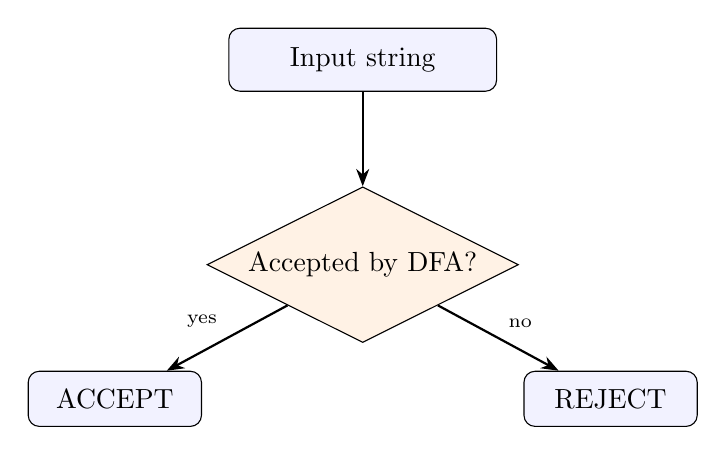
\begin{tikzpicture}[node distance=1.2cm]
  \node[block,minimum width=3.4cm] (start) {Input string};
  \node[decision,below=of start] (match) {Accepted by\ DFA?};
  \node[smallblock,below left=of match,xshift=-0.2cm] (accept) {ACCEPT};
  \node[smallblock,below right=of match,xshift=0.2cm] (reject) {REJECT};
  \draw[arrow] (start) -- (match);
  \draw[arrow] (match) -- node[above left,font=\scriptsize] {yes} (accept);
  \draw[arrow] (match) -- node[above right,font=\scriptsize] {no} (reject);
\end{tikzpicture}
\caption{TikZ illustration of the final DFA acceptance decision.}
\label{fig:result-decision}
\end{figure}

\section{Implementation and Usage}
The project is implemented in C++ and uses the Standard Template Library, including \texttt{std::string}, \texttt{std::vector}, and \texttt{std::set}. The code is separated into header files in \texttt{include/} and implementation files in \texttt{src/}. The PowerShell test runner is located in the project root as \texttt{tests.ps1}.

Compile from the project root with a C++ compiler such as g++:
\begin{lstlisting}[language=bash,numbers=none]
g++ -Iinclude src/*.cpp -o src/a.exe
\end{lstlisting}
Run the program on Windows using:
\begin{lstlisting}[language=bash,numbers=none]
.\src\a.exe
\end{lstlisting}
The program asks for a regular expression and then an input string. For automated testing, run the following command in PowerShell from the project root:
\begin{lstlisting}[language=bash,numbers=none]
.\tests.ps1
\end{lstlisting}

\section{Results and Testing}
The project includes a test script with 21 cases covering literals, concatenation, union, Kleene star, parentheses, nested expressions, a complex expression, empty input, and malformed expressions. The previously reported test run completed with all 21 cases passing and no failures. This is the recorded result from the development test run; rerun the script against the final submitted files to reconfirm it.

\begin{table}[htbp]
\centering
\caption{Representative functional test cases.}
\label{tab:tests}
\begin{tabular}{|l|l|l|}
\hline
\textbf{Regular Expression} & \textbf{Input String} & \textbf{Expected Result} \\
\hline
\texttt{a} & \texttt{a} & ACCEPT \\
\texttt{a} & \texttt{b} & REJECT \\
\texttt{a|b} & \texttt{b} & ACCEPT \\
\texttt{a*} & \texttt{aaa} & ACCEPT \\
\texttt{(a|b)*abb} & \texttt{abababb} & ACCEPT \\
\texttt{(a|b)*abb} & \texttt{ab} & REJECT \\
\texttt{(a|b)*abb} & \texttt{abc} & REJECT \\
\texttt{a|} & \texttt{a} & REJECT \\
\texttt{()} & empty string & REJECT \\
\hline
\end{tabular}
\end{table}

\subsection{Sample Console Interaction}
The following is a text representation of a sample run, not a screenshot of a live execution.
\begin{lstlisting}[language=bash,numbers=none]
Enter Regular Expression: (a|b)*abb
Enter String: abababb
Result: ACCEPT
\end{lstlisting}

\section{Limitations and Future Enhancements}
The current evaluator supports literals, concatenation, union, Kleene star, and parentheses. It does not currently implement advanced regex syntax such as character classes, escape sequences, optional matching, one-or-more repetition, or wildcard matching. The implementation also uses raw pointers for syntax-tree and automaton objects; smart pointers and explicit ownership management would improve memory safety. Possible future improvements include additional operators, clearer diagnostics for malformed patterns, memory-management improvements, and a visual display of NFA/DFA states and transitions.

\section{Conclusion}
The Regex Evaluator demonstrates the stages involved in implementing a basic regular-expression engine without relying on a built-in regex library. Recursive-descent parsing builds a syntax tree, Thompson's construction converts the tree into an NFA, subset construction produces a DFA, and DFA simulation checks the input string. The project applies abstraction, inheritance, polymorphism, encapsulation, and STL containers in a modular C++ implementation. The automated tests provide repeatable checks for supported operators and common invalid expressions.

\end{document}
